\section{Model of Computation}
\label{model}

The model we use for this paper is a general model that is agnostic of
input language.  The semantics of the model of computation employed in
this paper are built upon synchronous dataflow (SDF)~\cite{leeSDF}.
Although the model was inspired by the StreamIt programming language,
the model can represent aspects of other streaming programming
languages such as Brook~\cite{brook04}, Lime~\cite{lime10},
SPL~\cite{spl09} and SPUR~\cite{spur05samos}.  Consider a directed
graph $G = (V, E)$ corresponding to a streaming application. $F \in V$
is a filter in the application and $(f, g) \in E$ is an edge (or {\it
  channel}) in the graph that denotes communication from $f$ to $g$
using a FIFO channel.  Each filter is described by multiple rate
declarations, data reorganization patterns, and compute functions as
described below. The techniques in this paper require static-rate
graphs, i.e., all of the quantities of the filters are statically
determinable.

%  Figure~\ref{fig:streamgraph} gives an example
% stream graph for a FM radio with an equalizer.  The figure also
% includes details for two of the filters; the details are explained
% below.

% The filter is the basic unit of execution in our model.  Each filter
% is described by multiple rate declarations, data reorganization
% patterns, and compute functions.  Basically, each filter defines the
% number of items it consumers and produces each time it is executed.
% The execution of a stream graph is represented by a {\it schedule} of
% a graph $G$.  A schedule gives a multiplicity for each filter $F \in
% V$ that denotes how many times to fire filter $F$.  When a schedule is
% executed, each filter fires when it has buffered enough input to
% satisfy its input requirement (a filter will not fire more times than
% given by a schedule).  In our notation, a schedule is represented by
% the variable $\Sigma$, and it denotes a mapping from filters to
% non-negative integers. The multiplicity of filter $F$ in schedule
% $\Sigma$ is denoted by $M(\Sigma, F)$.

For each filter, $F \in V$, a {\it work} function, $W_F$, is defined.
The work function defines the atomic execution step for each filter.
When a filter fires, its work function is called once, consuming the
items and producing the items statically defined.  For each filter, $F
\in V$, a {\it prework} function, $W_F^P$, can also be defined.
Prework describes a computation step that executes once at the first
firing of a filter.  The prework function is executed only once per
execution of the {\it application}; it describes any special
initialization behavior required for a filter. We denote a function
with the variable $\mathcal{F} \in \{W^p, W\}$.  We sometimes leave
out the subscript that denotes the filter if it is clear which work or
prework function is intended.

For each filter $F \in V$ we define the following:
\begin{itemize}

\item $o(\mathcal{F}, F)$, the number of items dequeued from $F$'s
input buffer per firing of $\mathcal{F}$.  This quantity is termed the
{\it pop} rate.

\item $e(\mathcal{F}, F)$, 1 $+$ the greatest index that is read (but
  not necessarily dequeued) from $F$'s input buffer per firing of
  $\mathcal{F}$.  This quantity is termed the {\it peek} rate.

\item $u(\mathcal{F}, F)$, the number of items enqueued to $F$'s
output buffer per firing of $\mathcal{F}$.  This quantity is termed
the {\it push} rate.

\end{itemize}

\noindent Sliding window filters have a peek rate greater than the pop
rate.  We somethings refer to sliding window filters as {\it peeking}
filters. Figure~\ref{fig:pipeline-example}(b)
demonstrates a peeking filter.  The figures shows that the window of
items read for consecutive firings of the filter overlap.  For the
work function execution, a peeking filter $F$ requires $e(W_F, F)$
items to be on its input channel(s) to fire.  $F$ will consume
(dequeue) the first $o(W_F, F)$ items after the firing of the work function.

\begin{figure}[t]
\centering
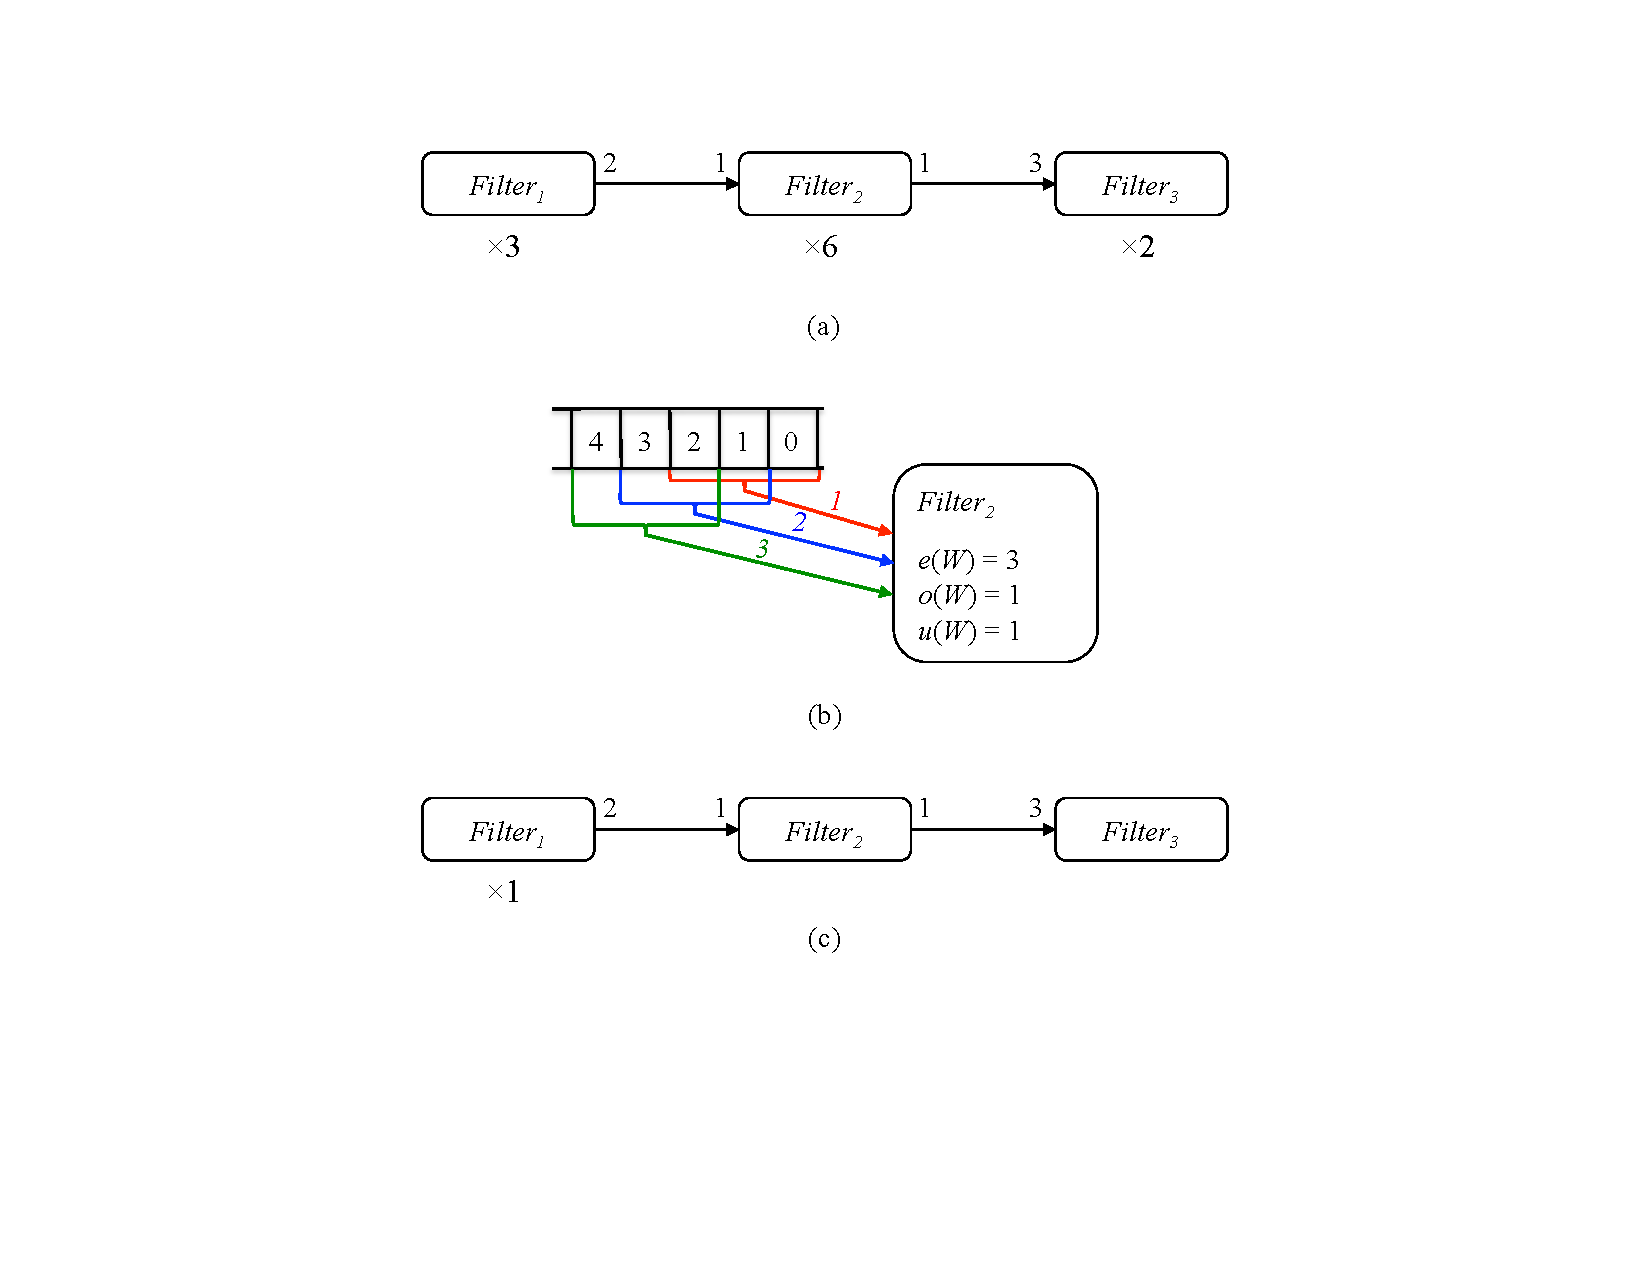
\includegraphics[width=3.0in]{figures/pipeline-example.pdf}
\caption[A pipeline of three filters with schedules.]{A pipeline of
  three filters.  In the figure, the number to the left of a filter is
  the number of items the filter consumes per firing; the number to
  the right is the number of items produced per firing.  (a) gives a
  legal steady-state schedule for the three filters.  (b) gives more
  detail for $\mt{Filter}_2$ including its peek rate.  The figure
  shows the window of items read for 3 consecutive firings of the
  filter.  Notice the overlapping in the windows.  (c) gives a
  legal initialization schedule for the graph that enables
  $\mt{Filter}_2$'s peeking. 
\label{fig:pipeline-example}}
\end{figure}


A schedule gives a multiplicity for each filter $F \in V$ that denotes
how many times to fire filter $F$. A {\it steady-state schedule} can
be calculated such that all filters fire in the schedule, and the
schedule can be repeated indefinitely~\cite{lee87}.  Steady-state
execution of the graph entails repeating the steady-state schedule for
as much input as is expected.  Due to this, execution of the stream
graph is conceptually wrapped in an outer loop that continuously
executes the steady-state schedule.
Figure~\ref{fig:pipeline-example}(a) gives an example of a
steady-state schedule calculated for a graph that consists of three
filters in a pipeline.  All the multiplicities of the steady-state can
be multiplied by the same constant $c$, and the result will still be a
valid steady-state.  We call this process {\it increasing} the
steady-state of the graph by $c$.

Our model does not deal with arbitrary schedules of filter executions.
The steady-state schedule, $S$, is explicitly represented.
Furthermore, an {\it initialization} schedule, $I$, is explicitly
represented that enables the steady-state schedule in the presence of
peeking filters.  Thus, in our model $\Sigma \in \{I, S\}$. 

An initialization schedule is required if peeking is present in a
graph to enable the calculation and execution of a steady-state
schedule~\cite{karczma-thesis}.  After the initialization schedule
executes, each filter $F$ is guaranteed to have at least $e(W_F, F) -
o(W_F, F)$ items in its input buffer. The initialization schedule is
required to calculate a steady-state schedule for a graph with an $F$
such that $e(W_F, F) - o(W_F, F) > 0$ (if the prework function peeks
then an initialization schedule is also
required)~\cite{karczmarek-lctes03}.
Figure~\ref{fig:pipeline-example}(c) gives a legal steady-state
schedule for the pipeline that enables the peeking in filter
$\mt{Filter}_2$.  During application execution, the initialization
schedule is executed once followed by an infinite repetition of the
steady-state schedule.   The number
of items remaining on $F$'s input channel(s) after execution of the
initialization schedule is represented by $C(F)$.  In the case of
Figure~\ref{fig:pipeline-example}, $C(\mt{Filter}_2) = 2$ and
$C(\mt{Filter}_1) = C(\mt{Filter}_3) = 0$.

A filter may have multiple incoming edges and/or multiple outgoing
edges.  Filter inputs are organized into a single internal FIFO buffer for the
filter to read according to an {\it input distribution pattern}, and
filter outputs are distributed from a single internal output FIFO
buffer according to an {\it output distribution pattern}.   
The input distribution pattern is represented as:

\[ \mt{ID}(\Sigma, F) \in (\mathbb{N} \times E)^n = ((w_1,e_1), (w_2,
e_2), ..., (w_n, e_n))\]

\noindent Where $n$ is the width of the input distribution pattern.
The input distribution describes the round robin joining pattern for
organizing the input data into the filter's single internal FIFO
buffer, where $w_i$ items are received from edge $e_i$ before
proceeded to the next edge, $e_{i+i}$.

The output distribution pattern describes both round-robin
splitting and duplication in a single structure:

\[ \mt{OD}(\Sigma, F) \in (\mathbb{N} \times (P(E)-\emptyset))^m = ((w_1,d_1), (w_2,
d_2), ..., (w_n, d_n))\]

\noindent Each $d_i$ is called the {\it dupset} of weight $i$.  The
dupset $d_i$ specifies that $w_i$ items be duplicated to the edges
of the dupset.  Each tuple denotes that $w_i$ output items of $F$ are
duplicated to the edges of $d_i$ before moving on to the next tuple.

\begin{figure}[t]
\centering
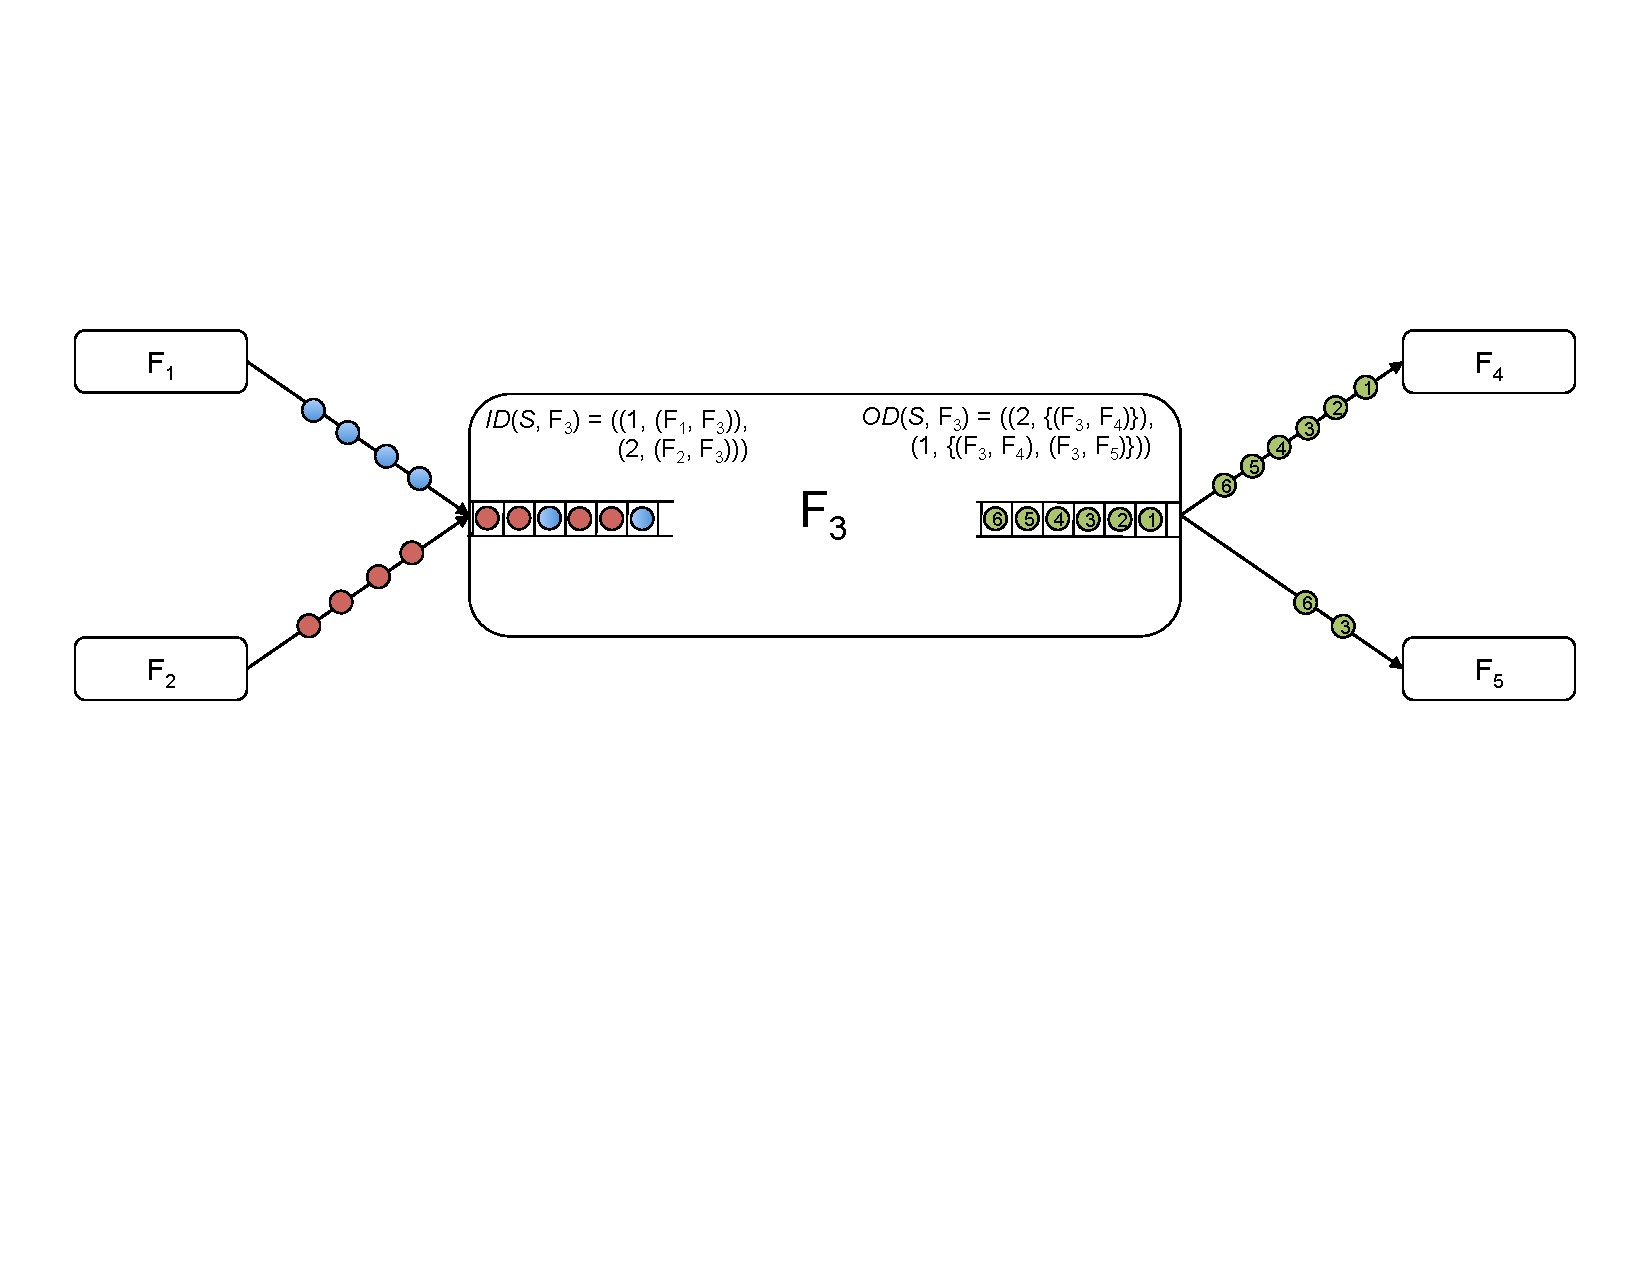
\includegraphics[width=3in]{figures/dist-example.pdf}
\caption[Example of input and output distribution.]{
An example of a filter with non-trivial input and output distribution patterns.
Filter $F_3$ has both multiple inputs and multiple outputs.  The input
items from the multiple inputs are joined in the pattern described by
its input distribution ($ID$): receive 1 item from $F_1$ and 2
items from $F_2$, and repeat.  $F_3$'s output items are distributed to
its multiple outputs as described by the output distribution pattern
($OD$):  2 items to $F_4$, then 1 item is duplicated to both $F_4$ and
$F_5$.  The output items of $F_3$ are indexed to show how they are
distributed to $F_4$ and $F_5$.
\label{fig:dist-example}}
\end{figure}

For both the $\mt{OD}$ and the $\mt{ID}$, the variable
$\Sigma$ specifies the schedule which the distribution pattern
describes, either $I$ for initialization, or $S$ for steady-state.
The input and output distributions are repeated as needed for the
schedule that is being executed.  The start of each steady-state
iteration resets the input and output distributions to the first tuple.
Figure~\ref{fig:dist-example} highlights an example of a filter with
both multiple inputs and multiple outputs, and how the distribution
patterns translate into scattering and gathering.

Let $\mt{RO}(F_1, F_2, \Sigma)$ be the ratio of output items $F_1$
splits along the edge $(F_1, F_2)$ to the total number of items that
$F_1$ produces in the schedule $\Sigma$.  This can be calculated from
$F_1$'s output distribution pattern for $\Sigma$.  For example, in
Figure~\ref{fig:dist-example}, $\mt{RO}(F_3, F_4) = 1$ and
$\mt{RI}(F_3, F_5) = \frac{1}{3}$.  Conversely, let $\mt{RI}(F_1, F_2,
\Sigma)$ be the percentage of total input items that $F_2$ receives
from $F_1$ for $\Sigma$.  For example, in
Figure~\ref{fig:dist-example}, $\mt{RI}(F_2,F_3) = \frac{2}{3}$.

% Let $s(\mathcal{F}, F)$ denote the execution time (in cycles, with
% respect to a given real or conceptual machine) of function
% $\mathcal{F}$ of filter $F$.  For many of the static scheduling
% techniques covered in this thesis, we calculate a static estimation of
% the total amount of work for a filter $F$ in the steady-state, $s(W,
% F) \cdot M(S, F)$.  We often use the term {\it work estimation} to
% denote this quantity.
